\documentclass{article}
\usepackage[utf8]{inputenc}
\usepackage{graphicx}
\usepackage{amssymb, amsmath, amsthm}
\usepackage{bbm}
\usepackage{biblatex}
\usepackage{floatrow}
\newfloatcommand{capbtabbox}{table}[][\FBwidth]
\addbibresource{references.bib}
\newcommand\numberthis{\addtocounter{equation}{1}\tag{\theequation}}
\usepackage[margin=1in]{geometry}
\graphicspath{ {report_figures/} }
\parskip = 0.1in

\begin{document}
\title{Rain}
\author{Matthew Wiens, Kelly Kung}
\date{December 20, 2017}
\maketitle
\begin{abstract}

Predicting precipitation is a key problem for residents of the Pacific Northwest, from it's impact on family vacations to landslides. A noteworthy feature of the area is distinct chances of precipitation between the summer and winter. In this report, we propose a model for differentiating the two seasons and understanding the chance of precipitation in each, across different climatic areas of the state. Such a model can be used to predict optimal times to travel from a rainy region to a dry region. We adopt a Bayesian methodology and  discuss predictive results within the Bayesian framework.  

\end{abstract}

\section{Introduction}

Residents and visitors to the Pacific Northwest (Oregon and Washington) notice a distinct pattern year over year: most days during the winter are rainy, and then they feel that there a distinct point during the spring or early summer when the weather becomes dry most days. Similarly, during early fall the nice weather switches back to rain.  However, the timing of the switch varies throughout the area, with the prominent Cascade Mountains being a key factor. There are many resorts on the east side of the Cascade Range that cater to residents of the west side looking to escape the rain. 

Widmann and Bretherton developed a methodology to control for local variation in topography and precipitation data and generated a dataset of estimated precipitation data over 46 years in a 50km by 50km grid.  In comparison, general models of atmospheric weather operate on the order of hundreds of kilometers, so there significant room to improve the spatial resolution of weather models.  In particular, local topographic features are not captured by general model, which is a limitation in regions like the Pacific Northwest.
The temporal and spatial correlation is also highly dependent on the topography and difficult to model, and therefore there has been a focus on parametrizing models and reducing the dimensionality. 


In this report, we propose a Bayesian approach for two reasons: first, to capture prior beliefs  from living in the area of one author, and second to be able to discuss distributions around complicated model parameters and probabilistic beliefs about the state of weather on a specific day of the year. Bayesian approaches for daily precipitation data are not new, for example see [Olson and Kleiber].  

\section{Background}

%Our Data

%Discussion of the areas
The Pacific Northwest has a varied climate, from temperate rainforests on the Pacific coast to desert in Southeastern Oregon, which has a major impact on the seasons. Therefore, each grid cell is classified into one of nine climatic zones as follows:
\begin{enumerate}
\item Washington Coastline (Temperate Rainforest)
\item Oregon Coastline
\item Western Washington / Seattle Metropolitan Area
\item Portland Metropolitan Area / Willamette Valley / Southwestern Oregon
\item Cascade Range
\item Columbia Plateau
\item Selkirk Mountains
\item Blue Mountains
\item Eastern Oregon / High Desert / Great Basin
\end{enumerate}
\begin{figure}[h!]
\centering
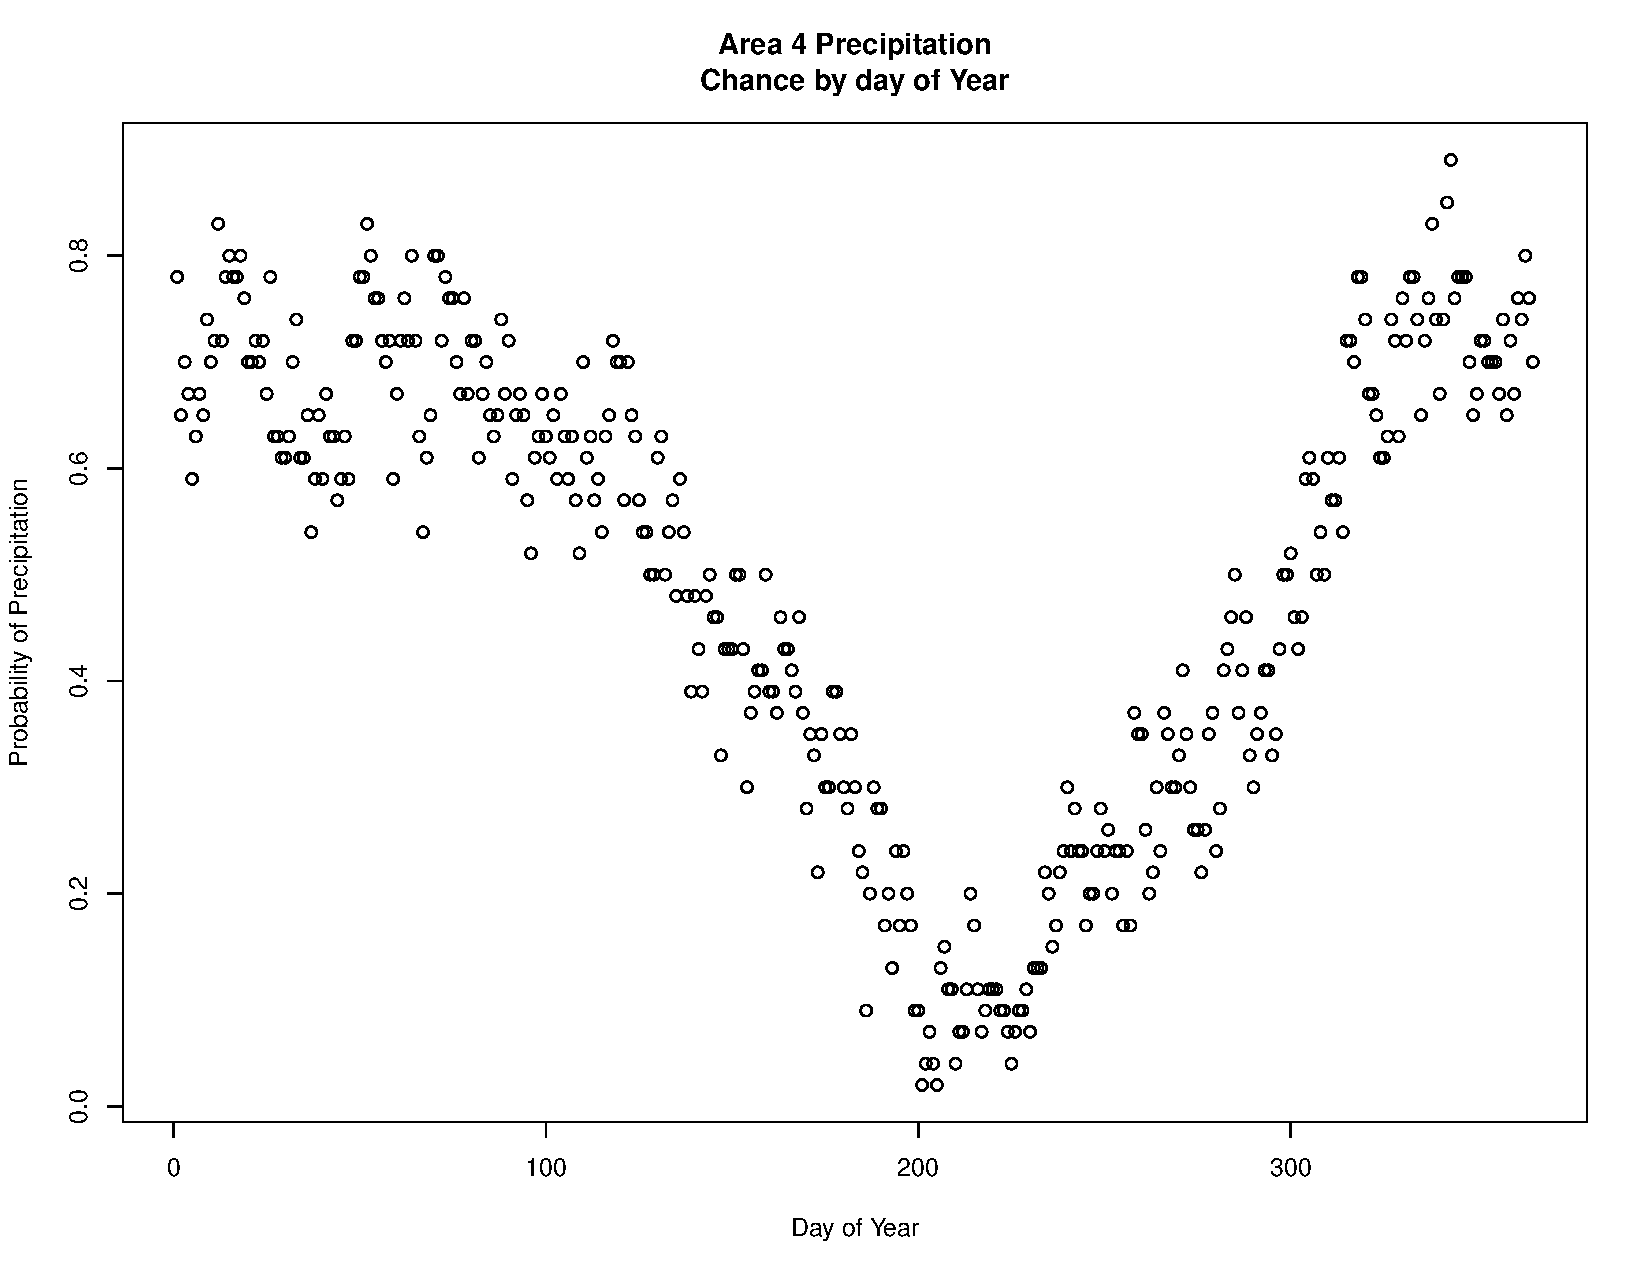
\includegraphics[width = .4\textwidth, height = 6cm]{Area4PrecipByDay}
\caption{Western Oregon precipitation chance over the year}
\label{fig:area4}
\end{figure}
These zones were decided by considering average precipitation over the time period of the data and the topographic features of the region. The rainfall for the region was aggregated by considering if there was measurable rainfall in each grid by day, and then for each day if the majority of grid cells reported rain, then a value of \textit{rain} was assigned to the area, else it was \textit{dry}


\begin{figure}[h!]
\centering
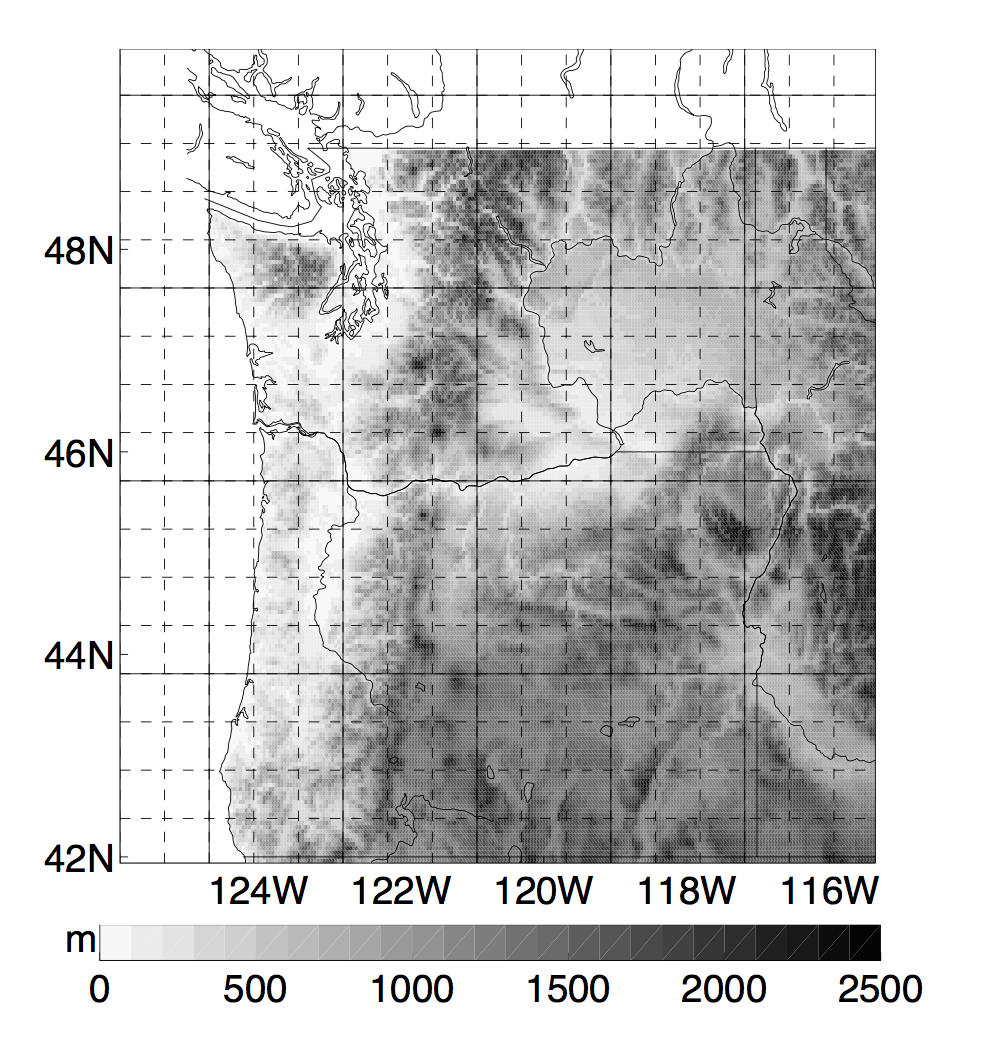
\includegraphics[width = .4\textwidth, height = 6cm]{topography}
\caption{Topography of the region }
\label{fig:area4}
\end{figure}
%The general problem we're trying to model

\section{Model}

%Maybe discuss first model here? It worked pretty well and informed future direction

We further developed our model by considering the probability of rain on each day for the summer (dry) and winter (rainy) seasons. This is motivated by the idea of trying to plan outdoor activity in each area of the Pacific Northwest and deciding if there is value in traveling to a different area to escape rain.
Therefore, the following model is proposed:
\begin{itemize}
\item The data is binary data representing if it rained or not for each day of the year,
\item $\pi_w$ and $\pi_d$ are the probability of rain during the wet season and dry season, respectively.
\item $\theta_1$ and $\theta_2$ are the cutoff points for the wet and dry seasons. The wet season runs from January 1st until the day before $\theta_1$ and from $\theta_2$ to December 31st, and the dry season runs from $\theta_1$ until the day before $\theta_2$, and the natural restriction is imposed that $\theta_1 < \theta_2$
\item Let $y_j$ be the data on day \textit{j}. Then $p(y_j) = \pi_w  1_{j < \theta_1} + \pi_d  1_{\theta_1\leq j < \theta_2} +\pi_w  1_{j \geq \theta_2} $
\end{itemize}

\section{Analysis}

\section{Discussion}

\section{Conclusion}
\end{document}